\chapter{Multi-agent reinforcement learning} \label{ch:marl}

\begin{chapter_outline}

In this chapter, we provide a broader overview of reinforcement learning.
We first introduce reinforcement learning in Section \ref{sec:ch2_Introduction} and define a stochastic game, the most common multi-agent framework, in Section \ref{sec:ch2_stochastic_Game}.
Multi-agent reinforcement learning is commonly divided into three settings described in Section \ref{sec:ch2_multi_agent_settings}.
Finally, in Section \ref{sec:ch2_single_agent_RL}, we provide essential details on the particular case of single-agent reinforcement learning where the foundations of multi-agent approaches reside.

\end{chapter_outline}

\section{Introduction} 
\label{sec:ch2_Introduction}
Reinforcement learning (RL) is a machine learning (ML) setting to solve decision-making problems.
We hereafter paraphrase several RL definitions.
Reinforcement learning is learning solutions of a sequential decision process by repeatedly interacting with an environment \citep{marl-book}.
Reinforcement learning is a kind of ML where an agent has to learn how to interact with its environment. \citep{pml1Book}.
Reinforcement learning is a framework for sequential decision-making, one core topic of ML \citep{introDeepRL}.
Reinforcement learning is a method to solve problems where decisions are applied to a system over time to achieve a desired goal \citep{BusoniuErnstBook}.
Reinforcement learning is learning by interacting in its environment to maximise a numerical signal called reward \citep{sutton2018reinforcement}.

In this 

multi-agent vs single-agent
Deep RL

define MARL and SARL

\section{Stochastic game}
\label{sec:ch2_stochastic_Game}
The stochastic game \citep{stochasticGames} is probably the most general framework in multi-agent.
In a stochastic game, a set of agents interact with the environment by observing the state of the environment, choosing actions and receiving rewards over a sequence of time, finite or not.
In this manuscript, we define a stochastic game by a tuple $[n, \mathcal{S}, \mathcal{U}, R, P, \gamma]$.
An agent is represented by $a$, and the set of agents is $\mathcal{A} \equiv \{1,..,n\}$.
We thus define each agent as $a_i$ with $i \in \mathcal{A}$ and any agent by $a$.

TODO: check state space vs set of 

At each time step $t$, each agent $a$ observes the state of the environment $s_t \in \mathcal{S}$ and selects an action $u_t^a \in \mathcal{U}^a$ with a probability given by its policy $\pi^a(u_t|s_t)$, where $\mathcal{S}$ is the state space, and $\mathcal{U}^a$ is the action space of agent $a$.
The joint action space is thereby $\mathcal{U} \equiv \bigtimes_{i \in \mathcal{A}} \mathcal{U}^{a_i}$, the joint action is $\mathbf{u} \in \mathcal{U}$ and the joint policy is $\mathbf{\pi}$.
As a consequence of the $n$ selected actions, the state of the environment $s_t$ transits to a new state $s_{t+1}$ with a probability $P(s_{t+1}, s_t, \mathbf{u_t})$ defined by the transition function $P:\mathcal{S} \times \mathcal{S} \times \mathcal{U} \rightarrow [0,1]$.

As the state transitions, each agent receives a reward denoted $r_t^{a_i} = R(s_{t+1}, s_t, \mathbf{u_t}, i)$ and defined by the reward function $R: \mathcal{S} \times \mathcal{S} \times \mathcal{U} \times \mathcal{A} \rightarrow \mathbb{R}$.
The goal of each agent $a_i$ is to maximise its expected sum of (discounted) rewards $\mathbb{E}_{\mathbf{\pi}}\left[ \sum_{t=0}^{T} \gamma^t r^{a_i}_t \right]$, where $T$ is the time horizon and $\gamma \in ]0, 1]$ the discount factor.
It is worth enforcing that the reward received by an agent is thus a function of the joint policy and not only of its own policy.
The time horizon $T$ defines the length of an episode, which is a complete sequence of actions in the environment and is considered finite in this work.
Finally, the discount factor $\gamma$ defines the importance of future reward.

Finding, or here learning, the optimal policy that maximises this expected sum is the purpose of reinforcement learning.
One solution is to find the Nash equilibrium.
TODO

Several comments can be addressed in the context of the work presented in this manuscript.
In the stochastic game definition, some include an initial state distribution which we keep implicit (e.g. \citep{marl-book}).
While the state space can be composed of discrete or continuous variables, the action spaces are considered discrete.
Agents do not always observe the entire state of the environment to select an action.
This is further developed in Section \ref{sec:ch2_partial_observability}.
In the literature, a stochastic game is also sometimes called a Markov game (e.g. \citep{MarkovGames}).

\section{Multi-agent settings} 
\label{sec:ch2_multi_agent_settings}
The stochastic game definition proposed in Section \ref{sec:ch2_stochastic_Game} provides a general framework for multi-agent systems.
By modifying the definition, it is possible to distinguish three main types of setting hereafter briefly described: cooperation, competition and general sum game.
In Section \ref{sec:ch2_single_agent_RL}, we develop details about a particular case, the single-agent setting.

\subsection{Cooperation} 
\label{sec:ch2_Cooperation}
When agents share the same goal, they cooperate.
Sharing the same goal means that a single reward function can be used instead of a set of reward functions \citep{}.
This adaptation of a stochastic game is one solution, and Part \ref{part:coop} of this manuscript is dedicated to cooperative settings with a common reward.
TODO: find another type of solution

Many problems can be modelled as a cooperative multi-agent setting.
TODO

\subsection{Competition} 
\label{sec:ch2_Competition}
When agents share completely opposite goals, they compete.
In competition, any action that benefits one agent incurs a retrofit to other ones.
This setting is most of the referred to as a zero-sum game \citep{}.
The property of a zero-sum game is that all rewards sum to zero at any time.
In a two-agent zero-sum game, commonly known as a two-player zero-sum in the game theory literature \citep{}, a possible adaptation of the stochastic game is to have a single reward function that one tries to maximise while the other tries to minimise it.

Many problems can be modelled as a competitive multi-agent setting.
TODO



\subsection{General sum game} 
\label{sec:ch2_general_sum_game}
The third setting includes everything that is not purely cooperative or purely competitive.
In this manuscript, we are interested in the mixed cooperative-competitive setting where two teams compete against each other.
Part \ref{part:compet} is dedicated to these settings, with the goal of studying how competition methods work in accordance with cooperation ones.
We can find several examples of such mixed cooperative-competitive settings.
TODO

Other types of general sum games exist, for example, when several agents have their own interests but share the environment with others.
TODO
traffic...


\section{Single-agent reinforcement learning} 
\label{sec:ch2_single_agent_RL}
As introduced, single-agent reinforcement learning (SARL) is the particular case of a multi-agent environment with a single agent.
Presented as such is a bit of a joke since the foundation of MARL relies on a lot of works first proposed for single-agent environments.
In this section, we will introduce the Markov decision process and how to learn an optimal policy, also referred to as the basics of reinforcement learning.

\subsection{Markov decision process} \label{sec:ch2_mdp}
By removing the agents of the stochastic game definition of Section \ref{sec:ch2_stochastic_Game}, we obtain the definition of a Markov decision process (MDP).
We therefore define an MDP as a tuple $[\mathcal{S}, \mathcal{U}, R, P, \gamma]$ where 

\begin{figure}
    \centering
    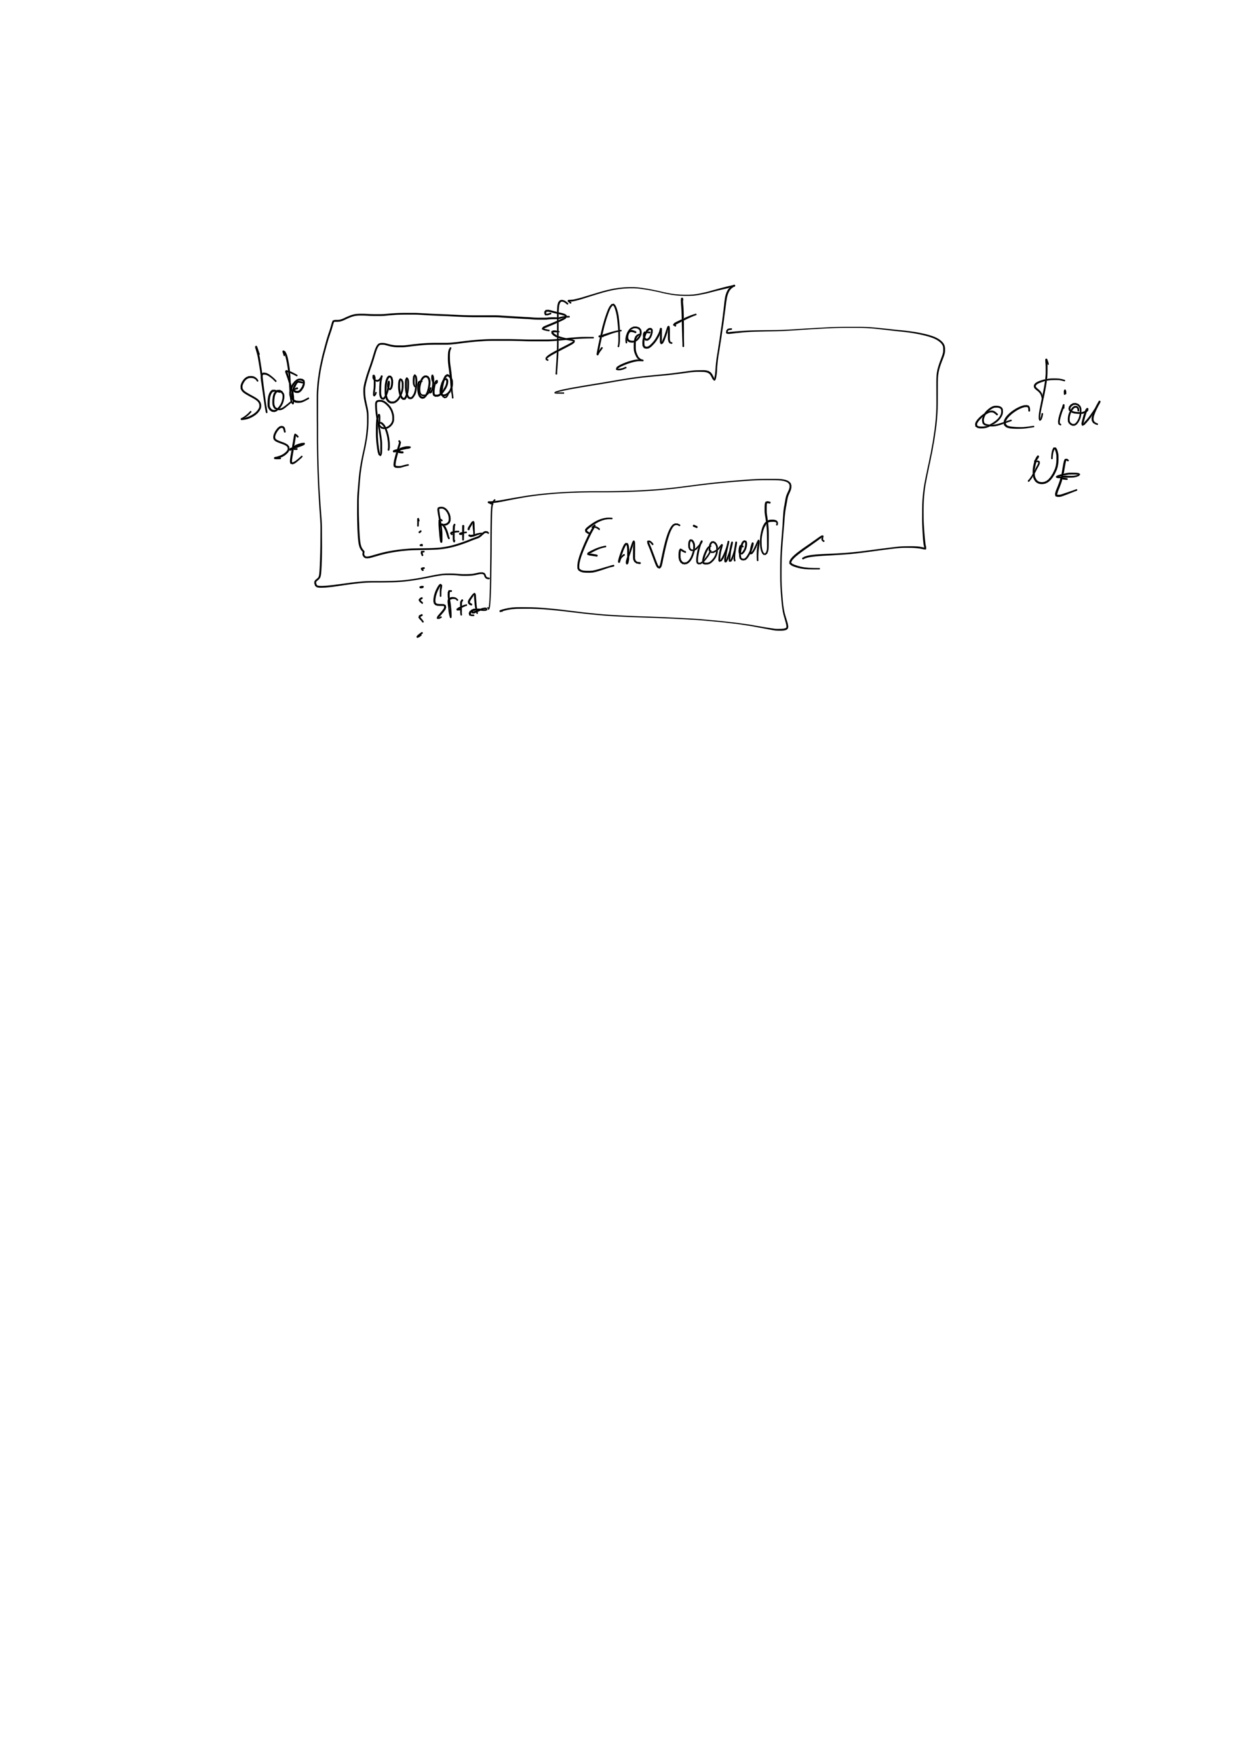
\includegraphics{tex_thesis/figures/ch2/mdp_sketch.pdf}
    \caption{Markov decision process \citep{sutton2018reinforcement}}
    \label{fig:ch2_mdp}
\end{figure}

\subsection{Model-based vs model-free} \label{sec:ch2_model_based_vs_model_free}
% Start from Moerland discussion + planning vs RL.
\subsection{Value-based methods} \label{sec:ch2_value_based_methods}
\subsection{Neural network} \label{sec:ch2_neural_network}
\subsection{Policy-based methods} \label{sec:ch2_policy_based_methods}
\section{Partial observability} \label{sec:ch2_partial_observability}
An observation function $O:\mathcal{S} \times \{1,...,n\} \rightarrow \mathcal{Z}$.
Agents sometimes store their history $\tau^a_t \in (\mathcal{Z} \times \mathcal{U})^t$.

\section{Further reading} \label{sec:ch2_futher}
